\begin{Exercise}[label = trinity, origin = Aaron Wild, title = {Project Trinity}, difficulty = 3]
	Die Ausbreitung einer halbkreisförmigen Schockwelle hängt von der Energie $E$ der Explosion sowie der Dichte der Luft $\rho$ ab.
	\Question Bestimme eine Gleichung, die den Radius $R$ der Schockwelle als Funktion der Zeit $t$ nach der Explosion angibt.
	\ExeText Die folgenden Bilder zeigen die Schockwelle nach dem ersten Atombombentest der USA 1945, \textit{Project Trinity}:
		\begin{figure}[h]
		\begin{subfigure}[b]{0.5\textwidth}
			\centering
			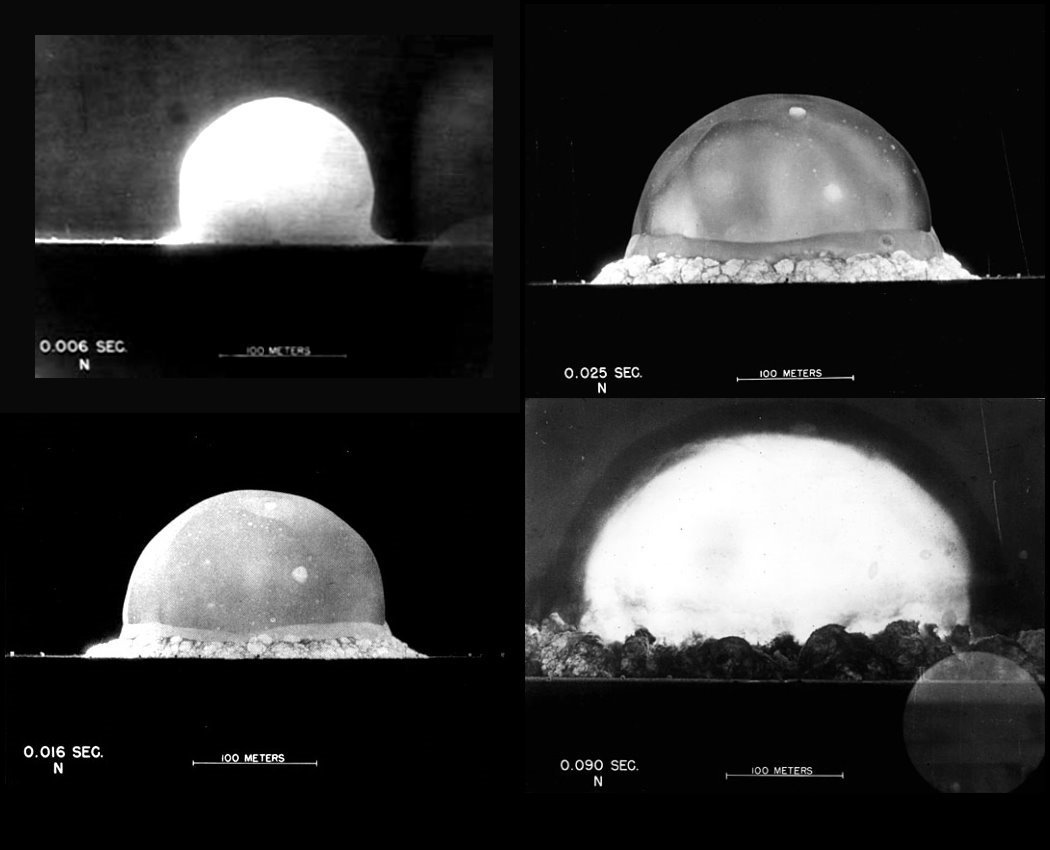
\includegraphics[scale = 0.25]{../tasks/selfmade/trinityim.png}
		\end{subfigure}
		\begin{subfigure}[b]{0.5\textwidth}
			\centering
			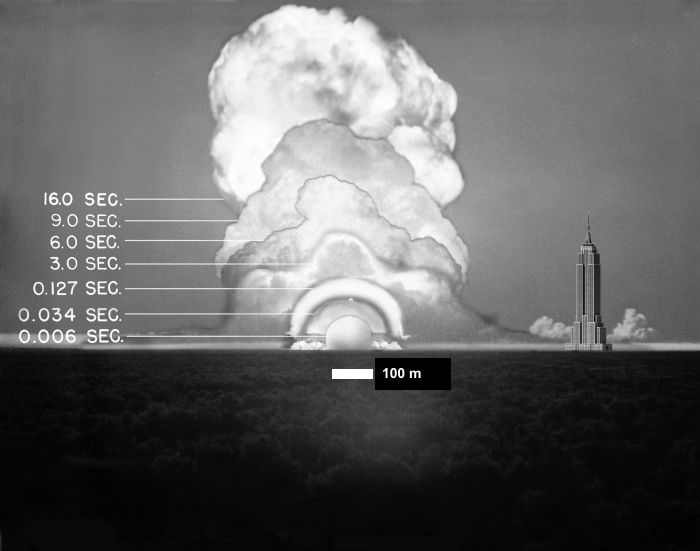
\includegraphics[scale = 0.25]{../tasks/selfmade/trinityim2.png}
		\end{subfigure}
		\caption{Massstabsgerechte Abbildung einer Schockwelle nach der Detonation}
		\label{fig:trinityim}
		\end{figure}
	\Question Nutze diese Bilder, um das Ergebnis aus 1. zu bestätigen.
\end{Exercise}
